\documentclass[a4paper]{article}
\usepackage{titlesec}
\usepackage{graphicx}
\newcommand{\sectionbreak}{\clearpage}
\renewcommand{\figurename}{Obr.}

\usepackage{times}

\usepackage{hyperref}


\usepackage{lingmacros}
\usepackage[document]{ragged2e}
\usepackage{booktabs} 

\usepackage{graphicx, float} 
\graphicspath{ {pics/} }

\begin{document}
\section*{VYSOKÁ ŠKOLA\\UMĚLECKOPRŮMYSLOVÁ V PRAZE}
Tvorba písma a typografie\\
Bakalářská práce\\
Jan Šindler\\
\vspace{20mm}
Písmo pro digitální zobrazování\\
\vfill
Praha, 2019\\
Vedoucí bakalářské práce: Tomáš Brousil\\
Konzultant bakalářské práce: xxxx\\

\section{úvod}
Téma jsem si vybral hlavně kvůli vlivu stáže ve firmě LucasFonts v létě 2018. Při stáži jsem se dozvěděl spoustu nového a zjistil jsem, že naše praxe není pouze o tvarování křivek. LucasFonts se věnují navrhování a produkci těch nejkvalitnějších fontu, které vydrží spoustu let. Rád jsem byl součástí týmu a doufám, že zase někdy budu. Poprvé když jsem od Lucase slyšel magická slova jako VTT a hinting, tak jsem mohl pouze předstírat, že vím o čem je řeč. První pokusy s hintingem proběhly už na stáži, šlo především o pokus-omyl metodu aplikování hintingu, moc jsem si z toho neodnesl. Po stáži jsem se začal věnovat oborům jako je programování a začal jsem se zajímat o strukturu fontového souboru. Hinting pořád neodmyslitelně patří k písmové produkci a je škoda, že o tomto řemeslu už moc lidí neví. Je důležité znát jeho sílu abychom mohli lépe navrhovat a uspokojit nejen svojí neukojitelnou autorskou touhu ale i koncového spotřebitele. O hintingu chci mít hlubší ponětí abych mohl dělat lepší písma, znát okolnosti a získat výhodu na trhu práce. Během studia jsem žil v naivní představě o nadvládě tvarosloví nad vším ostatními odvětvími navrhování písma, už to tak není a svou bakalářskou prací posouvám tvarosloví dané beziérovými křivkami ještě dále. Budu zpracovávat písmo, které bude vycházet z dat, které představuji dále v mé bakalářské práci. Zajímá mě hlavně vztah bitmapové rasterizované kontury a kontury samotné. Kdy se stane to, že naše milované písmo ztratí všechno co jsme mu dali a jeho z něho pár pixelů? Mohu navrhnout písmo, které bude vycházet z omezení mřížky, do které se navrhuje a nevypadalo jako z 90. let? Chci udělat písmo pro 1bitové displeje, protože právě pro tyto systémy vidím hinting jako obrovský potenciál. Chci navrhnout alternativu k písmu Verdana a Tahoma, která bude nabízet trošku jiný pohled na věc a bude stejně dobře zpracovaná. Samotná teoretická práce se zabývá analýzou situace ve světě digitálních písem, a přehledem nad tzv. big daty, které jsem sesbíral a analyzoval. Výsledky analýz jsou fakta, na kterých zakládám svůj projekt.

\section{Co je to vlastně hinting?}

Hinting je optimalizace TrueTypových a nebo PostScriptých fontů k docílení co největší čitelnosti a nebo naplnění jiného požadavku. Hint je v překladu nápověda, hinting je tedy jakési dávání rad rasterizéru, který je hloupý a bez rad by písmo dobře nezobrazil. 


\subsection{Hinting dnes}

je umírajícím řemeslem, pro většinu případů stačí auto-hinting, v dalších případech o tento aspekt fontu designér nejeví zájem protože pracuje na zařízení s vysokým rozlišením. To se projeví až u koncového uživatele. Nutno přiznat, že hinting není tak potřeba jak dříve pro užití na stolních počítačích. Dokonce i já jako středoevropan s poměrně výkonným počítačem si všímám nekvalitně udělaných písem na webu, ty pak často velmi znepříjemňují čtení na digitálních zařízení. Jsou profese, u kterých lidé stráví několik hodin denně u počítače, na čitelnosti záleží a nemůže dojít k sebemenšímu omylu. Příkladem může být například opensourcové písmo Fira, které je velmi rozšířené mezi programátory.  Uživatelé si nesprávného hintingu všímají a i když často neví, jak tento problém pojmenovat tak ho nahlásí tvůrci písma aby jej \href{https://github.com/tonsky/FiraCode/issues?utf8=%E2%9C%93&q=hinting}{opravil}. Nesmíme si dělat iluze, že hinting nikoho nezajímá. Kde se vlastně vzala tahle nálada, když věnujeme takovou péči písmu pro tisk?


\subsection{Druhy Hintingu detailně}

\begin{enumerate}
\item \textbf{TrueTypový hinting}
je velmi silný nástroj, který umožňuje modifikace písmen u každé velikosti a to do těch nejmenších detailů, jako posunutí bodu pro určitou písmovou velikost klidně i o 1/16 pixelu. Nástroj je to silný a jeho ovládání je velmi komplexní. TT hinting jak ho známe dnes si můžeme představit jako vizuální programování, kde nastavujeme pravidla. Je nutno si uvědomit, že je to programovací jazyk a každý znak má program v takovémto jazyku k sobě přiřazen, který komunikuje s rasterizérem a radí mu jak se vykreslit, pak je už na samotném rasterizéru jak s takovýmito radami naloží.

\item \textbf{PostScriptový hinting}
Postcriptový hinting je modernější forma hintingu, je jednodušší než TrueTypový ale neumožňuje takové modifikace.

\item \textbf{Autohinting}
 je automatické vytvoření hintingového programu pro písmo. TrueTypový může fungovat buď na základě postscriptového hintingu (bude fungovat přesněji než kdyby se algoritmus pokoušel o automatizaci hintingu bez něj). TT autohinting může narazit v případě kdy jde o nestandartní písmo, například když konce tahů nekončí přímo na dotažnicích. Autohinting taky nemůžeme aplikovat na písma, kde je důležité vědomí o souvislostech v písmu. To jsem už sám pocítil při práci na variabilním písmu, kde jsem mohl hintovat pouze v ose Y. To by nebyl takovým problém sám o sobě, písmo působí efektem 3D rotace a při pohledu z 90 stupňů se začnou překrývat a kontura se začne zaokrouhlovat na rozdílné strany, to vytváří na kontuře nepříjemné schody. V normálni situaci by tohle hinting vyřešil, jelikož ale chceme plynulou animaci tak v ose X žádný hinting aplikovaný být nemůže, kontura se vymění za obdelník stejných rozměnu přesně při devadesáti stupních, při pohledu ze strany tedy na kontuře nevznikají žádné schody. Aby přechod mezi znaky a obdelníky byl plynulý, musí i tyto obdelníky být vyhinitované stejně jako znaky, které zastupují. Stroj tyto souvislosti neví a tak bylo potřeba toto písmo vyhintovat ručně.
\end{enumerate}

\section{programy okolo hintingu}
neco napsat o programech obecne

\subsection{VTT}
Link - základní nástroj pro, kterým určujete jaký vztah jeden kotevní bod naplňuje k druhému. Může jít o jednoduchý pohyb - pohne-li se jeden, pohne se i druhý a nebo že tyto dva body budou od sebe vzdáleny stejný počet pixelů jako druhé dva body. Delta – posouvání buď globálních a nebo lokálních hodnot - nastavíme li že všechny body na x-výšce jsou označeny číslem 6, nástrojem delta můžeme určit v jakých velikostech se případně výška o bod zvedne, nejsme-li spokojeni s plynulostí gradace velikostí. Lokální deltou pak ovládáme body stejným způsobem a to od nejjemnější nuance 1/8 bodu až po 8 bodů do plusu i záporu, pokud by to mělo nějaký důvod, můžeme nastavit, že písmeno 'o' je širší nebo užší až o 8 bodů ve zvolené velikosti. Interpolate - interpoluje jeden bod na základě dalších dvou – něco jako když na pružinu umístíme bod a pak s jí natahujem, bod bude vždy ve stejném vzdálenostním poměru ke krajům pružiny.

\subsection{rasterizéry}
\begin{enumerate}
\item ClearType - rasterizer Windowsu, funguje na bázi rozdělení pixelu na sub-pixely. RGB = 1 pixel, R = 0.33 pixelu

\item FreeType - opensourcový projekt, který najdeme ve velkém množství zařízení. Od Androidu/Linuxu až po telefony společnosti Apple. Jde o opensourcovou variantu ClearTypu

\item Quartz - rasterizer MacOs, ten ignoruje veškteré hintingové instrukce a rastr vytvoří podle vlastního algoritmu, tak aby text vypadal na obrazovce co nejvíce jako jeho tištěná podoba. To má za důsledek, že písma jsou velmi špatně čitelná v malých velikostech.

\item CoolType - je metoda rastrování textu, kterou využívá Adobe a jejich řada programů
\end{enumerate}

\section{analýzy}
Proto abych lépe pochopil data okolo fontů a digitální stopu, kterou ve světě zanechávají, tak jsem použil služby od Googlu se jménem BigQuerry. Ta umožňuje prohledávat ohromné množství dat za pár vteřin. BigQuerry navíc nabízí svoje vlastní datasety a to zdarma. Já využil hlavně datasetu od githubu, zajímalo mě hlavně v jakém poměru se používají patkové a nepatkové písma na webu a také jaká velikost písma je nejpoužívanější.
\subsection{font-size}
Obrazovky se dnešních počítačů v Evropě a dalších rozvinutých zemích problémy se zobrazováním písma skoro nemají, nesmíme ovšem opomíjet země, kam naše technologie ještě nedorazila a navrhovat písmo i pro ně. Velké firmy by měly mít písmo, které obstojí v jakékoliv situaci a to i na tom nejslabším zařízení. Typickým příkladem může být displej pračky, digitální cenovka v supermarketu a nebo jednoduchý počítačový systém, který nepodporuje nejmodernější zobrazovací technologie, příkladem může být platební terminál. Všechny tyto zařízení vyžadují buď aplikace firemních písem, log a nebo piktogramů. Zde všude může hinting velmi pomoci. Písmo jsem navrhoval primárně pro nějakou velikost, která je lidmi nejpoužívanější, svůj požadavek jsem zadal pouze na webové nastavení, hlavně protože je ustálené a programátoři velikost vybírají s vědomím, že neví na jakém zařízení se jejich web zobrazí. Jelikož jde o akademický úkol, tak ani já nevím na jakém zařízení bude moje písmo zobrazováno. O to zajímavější to je, neboť mi jde o to aby vypadalo, četlo se a fungovalo dobře na všech zařízeních. Pro mojí analýzu jsem využil služby BigQuery od Googlu, která dovoluje zkoumat velká množství dat pomocí jejich počítačů. Data jsou buď externí a nebo přímo od Googlu, takový soubor dat se nazývá dataset. GitHub je platforma pro vývojáře, kde si lidé mohou ukládat a sdílet právě vyvíjenou aplikaci buď mezi sebou a nebo mezi veřejnost. Jeden z datasetů githubu má 2,3TB, já jsem svůj pokus dělal pouze na neplacené části 30GB a i tak jsem dostal velké množství dat, kterou jsou svojí kvantitou dostačující. Programátoři využívají z velké části jednotky PX oproti PT, které jsou určené spíše pro tištěné výstupy. Z dat vyplynulo, že nejpoužívanější velikostí pro weby je 14PX a 10PT což se rovná 13.3PX. Základní velikostí pro navrhování písma určeného k digitálnímu zobrazování je tedy velikost 14PX. To je velikost, kde se právě začínají lámat rozdíly mezi hintingovými unibody písmy a písma se už začínají lišit. Mřížka B/W monitoru je omezena a proto mohou působit nějaká písma dost podobně i když jde původně buď o egyptienkové písmo a knižní serif. V případě malých velikostí ovšem nemůže jít o to se odlišit ale zaručit, že písmo bude fungovat i v malých velikostech. Nemluvě o přizpůsobení piktogramů a log k takovýmto zobrazení.

\begin{tabular}{r|rrr}
jednotka & \\
& medián & \\
& & m. průměr & \\
& & & počet nálezů\\
\midrule
PX & 14.0 & 26.8330 &13352 \\
PT & 10.0(13.3330PX)  & 12.3086 & 1231 \\
EM & 1.2 & 3.0410 & 7225 \\
\% & 100.0 & 114.9932 & 6295\\
\end{tabular}

\subsection{font-family}
Mým dalším cílem zkoumání pomocí služby BigQuery bylo i jaké písma uživatelé používají. Vysledky ukazují, že převažují písma bezserifová a většinou systémová. Z toho vyplývá, že programátoři jsou si vědomi výhod takových písem. Systémová se nemusí zobrazovat a bezserifová jsou lépe čitelná na obrazovkách nižších rozlišení. Těmito dvaceti nejpoužívanějšími fonty je pouze jedno serifové, velmi překvapivé je, že Times New Roman se do téhle dvacítky vůbec nedostal. Zdali absence patkových písem je následkem slabé nabídky a nebo zkrátka nejsou určena pro digitální formu zobrazování je na diskusi. Fonty se pro weby nastavují buď konkrétně a nebo jako skupina, tedy název fontu – Arial – nebo druh fontu - Sans Serif. Font se nemusí nastavit jenom jeden v případě, že by font na cílové mašině nebyl, nahradil by se nekontrolovatelně na základní font platformy. To nechceme a proto můžeme v pořadí naších preferencí nastavit fonty dle libosti, pokud první v systému není, aplikuje se ten další atd. příklad font-family="Arial, Helvetica, Verdana".

\begin{tabular}{r|rlr}
název písma/skupiny & \\
& počet nálezů & \\
&& distribuce&\\
\midrule
sans-serif & 25895 &  Skupina\\
Arial & 20070 & WIN\\
Helvetica & 11886 & MAC\\
Helvetica neue & 6560 & MAC\\
Verdana & 5618 & WIN\\
monospace & 4881 & Skupina\\
Courier & 4315 & WIN\\
Tahoma & 2953 & WIN\\
inherit & 2943 & Skupina\\
Lucida console & 2239 & WIN\\
Font Awesome & 2163 & ID\\
serif & 2146 & Skupina\\
Lucida grande & 1733 & OS X\\
Monaco & 1413 & OS X\\
Lato & 1191 & G\\
Open sans & 1135 & G\\
Courier new & 1119 & WIN\\
Consolas & 1099 & WIN\\
Georgia &  1038 & WIN\&MAC\\
Segoe ui & 819 & WIN\\
\end{tabular}

\section{Pixel a pixel mimo digitální svět}
rastr vektoru - pixelizaci nesmíme striktně chápat jako něco co se vyskytuje výhradně na obrazovkách, jde o rozložení křivek na pravidelnou mřížku. O pravidelnou a ovladatelnou distribuci bodů křivky na tom rastru nám jde především když je velikost mřížky omezena. Uvádím zde tři příklady, kdy se taková distribuce hodí i pro aplikace jiné, než je obrazovka.\\

\begin{enumerate}
\item \textbf{Jehličkové tiskárny} s povinností tisknout všechny účtenky, roste i spotřeba thermopapíru, ten je ovšem nerecyklovatelný a na tento fakt často ochránci životního prostředí poukazují. Obchody, které jsou s touto problematikou obeznámeny používají staré jehličkové tiskárny, protože jde o tisk barvou na recyklovaný a dále recyklovatelný papír.Jde o jakýsi trend, který se šíří napříč bioobchody a kavárnami, řeší problém s nerecyklovatelnými thermopapíry a ukazuje nám, že žádná technologie není mrtvá a je velká šance, že se jednou či později opět vrátí. 

\item \textbf{Práce se samotným pixelem}
obrázek není jenom sled obrázku a bodů ale přesná mřížka s přesnými údaji, to v dnešní době můžeme využít a můžeme pracovat se samotnými pixely. I trošku zruční designéři jsou už schopní si vyrobit vlastní rasterizer, který bude tvořit například vizuál pouhým festivalu aplikováním rasterizeru na fotografii. To nám skvěle předvedl například Just van Rossum a Hansje van Halem při vizuálech na vizuálních stylech festivalů Lowlands a nebo studio Norm při navrhování nové podoby švýcarských bankovek. Pokud mám pole typu šachovnice o veliksoti 2x2 pixelů, data obrázku by vypadala asi takto [[255, 0], [0, 255]]. S daty pak můžeme libovolně pracovat. Můžeme například všechna políčka, kde je bíla (255) spojit čárou a nebo je nahradit nějakým symbolem. Můžeme je nahradit třeba obličeji politiků, síť by pak byla asi v mnohem větší velikosti, než bychom očekávali od obrázku s rozlišením 2x2 pixelů. Z tohoto obrázku se nyní stává síť, kde každý bod může být pozorován samostatně. Dohromady však tvoří celek, kde rovnoměrná distribuce je důležitá.

\item \textbf{Průmyslová produkce návrhů}
jsou technologie, kdy při realizaci návrhu je míra detailu velmi omezena. Typicky může jít o pletení, tkaní, vyšívání a nebo perforace do nejrůznějších materiálu.
\end{enumerate}

\subsection{\textit{O} u Timesu je stejné jako u Arialu}
Unikátní tvar písmene, který jsme zvyklí posuzovat z papíru a jsme na něj tak pyšní se na obrazovkách promění a je z něho něco o čom jsme vůbec netoužili. V těch nejmenších velikostech naše výmysly zanikají, písmo je nečitelné a my jsme naštvaní. Hinting zaručí čitelnost i v těch nejmenších velikostech. Při mřížce, která může být vysoká vysoka i třeba jen 20 bodu zanikají ty nejmenší detaily a jedno písmo začíná připomínat to druhé. Jestli si někdo myslí, že tvorba písma o tom dělat písmena jinak, než ty před námi, tak se mýlí. Jestli jsou písma opravdu identická zkoumám v následujícím pokusu. Porovnávám bitmapy u písmen arial.ttf, georgia.ttf, tahoma.ttf, verdana.ttf, consola.ttf , lucon.ttf a times.ttf ve velikostech 8, 9, 10, 11 a 12 pixelů v jednobitovém režimu zobrazování.\\
\begin{tabular}{r|cccccccccccc}
\rotatebox[origin=l]{90}{počet shod}&
\rotatebox[origin=l]{90}{shodné písmeno}&
\rotatebox[origin=l]{90}{písmo a velikost}&\\
\midrule
5 & o & A 9 & o & G 9 & o & Ta 9 & o & Ti 9 & o & Ti 10\\
4 & O & A 9 & O & Ti 9 & O & Ti 10 & 0 & Lu 11\\
4 & 8 & A 9 & 8 & G 9 & 8 & Ta 9 & 8 & Ti 10\\
3 & i & A 8 & l & A 8 & I & A 8\\
3 & D & A 8 & D & Ta 8 & D & Co 10\\
3 & e & A 9 & e & G 9 & e & Ta 9\\
3 & t & A 9 & t & Ti 9 & t & Ti 10\\
3 & j & G 9 & j & Ti 9 & j & Ti 10\\
3 & l & G 9 & l & Ti 9 & l & Ti 10\\
3 & u & G 9 & u & Ti 9 & u & Ti 10\\
3 & 0 & Ta 9 & 0 & Ti 9 & 0 & Ti 10\\
3 & e & G 10 & e & Ta 10 & e & Ti 11\\
3 & 0 & G 10 & o & Ta 10 & o & Ti 11\\
3 & o & G 11 & o & Ta 11 & o & Ti 12\\
\end{tabular}
\vspace{20mm}\\
A=Arial, G=Georgia, Ta=Tahoma, Ti=Times, Lu=Lucida Console, Co=Consolas\\

\section{návrh písma Delta}
Po všech těchto průzkumech a pochopení problematiky jsem teprve mohl začít navrhovat konturu. Potenciál pro využití této technologie vidím hlavně u velkých firem, kde není známo kde všude se jejich písmo může objevit. Chci nabídnout alternativu k písmu Verdana, která bude odrážet vizuální kulturu dnešní doby a bude stejně kvalitné přizpůsobena jednobitovým displejům. Při hledání písma pro takové displeje jsme velmi omezeni a pravděpodobně nejčastěji stejně skončíme u Verdany. To je klasické písmo a nemůže si dovolit být trochu expresivnější protože jde o celosvětový projekt. Proces mé tvorby popisuji chronologicky.
\subsection{Konzultace}
Na fóru TypeDrawers jsem narazil na písmového inženýra – Mika Duggana, byl velmi ochotný se mnou konzultovat a vysvětlil mi nejzákladnější principy, které člověk aplikuje při hintování písma. Mike pracuje v Microsoftu a má za sebou hintování například písma Times New Roman.
\subsection{Mřížka a kontura v ní}
Při navrhování samotné kontury jsem chtěl vycházet z omezení daných tou nejpoužívanější mřížkou, tedy jak data ukazují, mřížkou o velikosti 14px. Právě velikosti okolo této by měly být ty nejpoužívanější. Omezení, která určuje by se měly promítnout do finální podoby kontury, aby originální kontura neztratila svou originalitu ve své bitmapové verzi. Skicoval jsem si do čtverečkovaného bloku a nebo kreslil rovnou v počítači v jednobitovém režimu. Doufal jsem, že najdu tímto způsobem něco unikátního a písmo v jednobitové aplikaci bude velmi připomínat to, které známe v tištěné podobě. Pro výšku x jsem vymezil 8 bodů, verzálky jsou o 2 body vyšší a spodní dotažnice o 2 body nižší, horní dotažnice je pak o jeden bod vyšší než verzálky. Rozdíl mezi výškou x a verzálkami o právě 2 body je důležitý pro primární velikost 14px hlavně kvůli identičnosti kontur napříč verzálkami a mínuskami v této velikosti. Rozlišení mřížky přenesl do mřížky fontu, tak že jeden čtverec mřížky má rozměry 44*40. Dřík má tedy tloušťku 44 bodu a horizontální tah 40. Písmo je navrhováno do několika kuželek, nejčastěji o šířce 4-6 bodů. Což vychází z faktu, že písmena v těchto kuželkách při 1bitovém zobrazování skončí, tak proč je tak nenavrhnout rovnou?
\subsection{Bezpečné úhly}
pro rovnoměrnou distribuci pixelů na diagonálách je velmi důležitý úhel ve kterém diagonály jsou. Úhel je úhlem diagonály obdelníku s poměrem stran 1:x. U 1:1 to je 45 stupňů, u 1:2 to je 26.5 atd. Tento tvar pak vyplňuje konturu, buď stoupa po jednom bodu doprava a nahoru a nebo o jeden doprava a dva nahoru.
90,
45,
26.5 a 
18.5 stupňů jsou nejpoužitelnější úhly pro obrazovku. V mém písmu se snažím všechny diagonály přizpůsobit těmto úhlům. Mezi 45 a 26.5 je poměrně velký rozdíl a když diagonála nespadá ani k jednomu z těchto úhlů, tak používám umělý bezpečný úhel, tzn. například úhel obdelníku 1:x.5. Ve velmi ojedinělých jsem byl přinucen bezpečný úhel vypustit. 

\begin{figure}[H]
  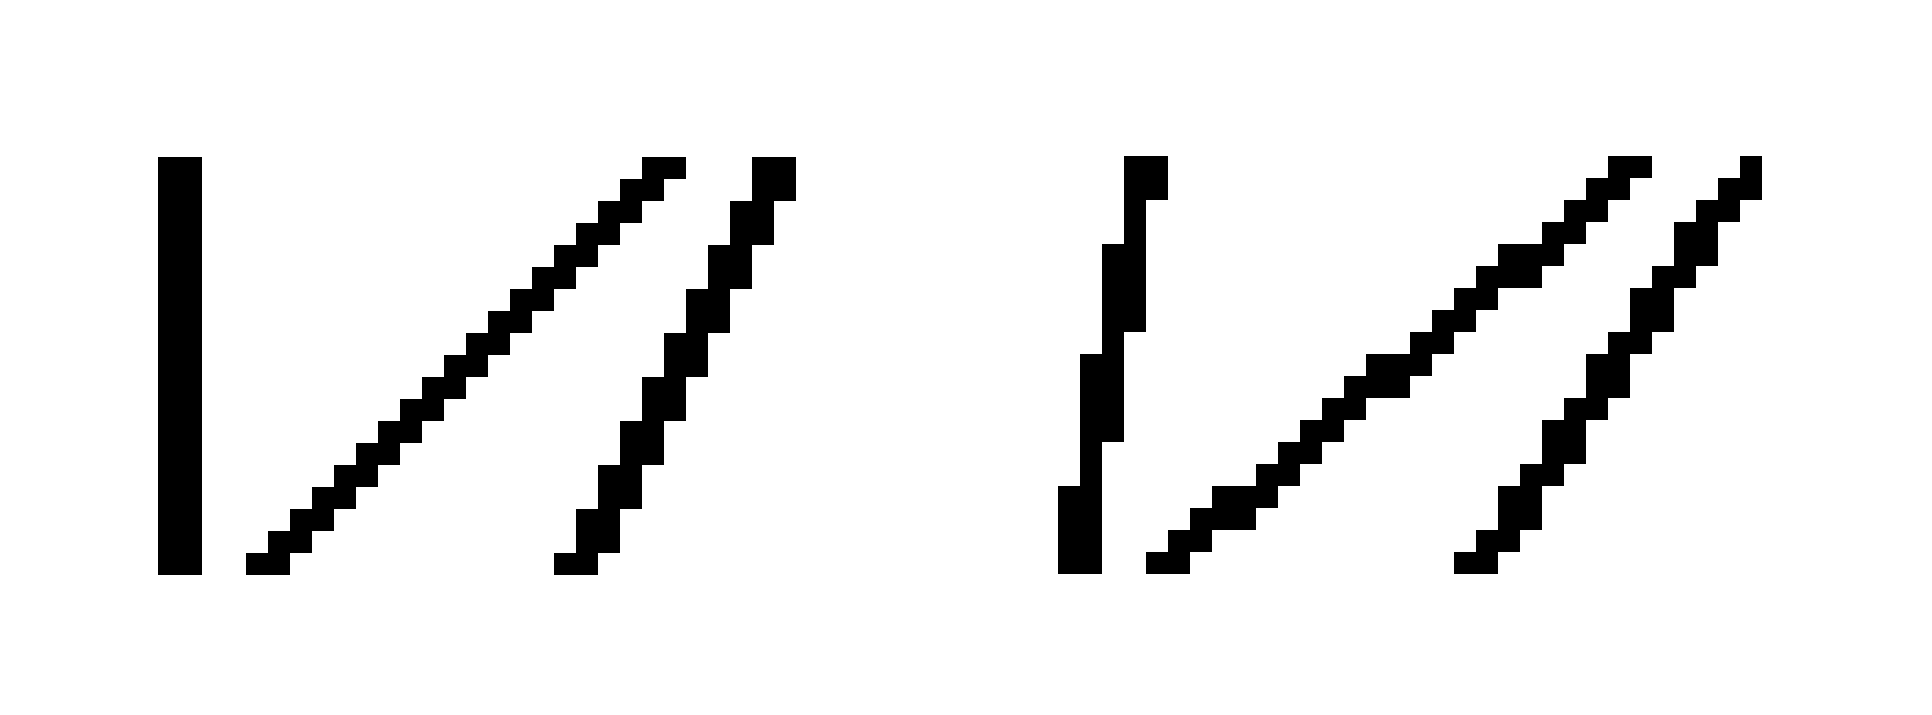
\includegraphics[width=\linewidth]{pics/1bit.png}
  \caption{vlevo tři diagonály pod úhlem 90, 26.5 a 18.5 stupňů, vpravo totéž ale vše o 10 stupňů zkoseno doprava. Jednobitové renderování}
\end{figure}

\begin{figure}[H]
  \includegraphics[width=\linewidth]{pics/bw.png}
  \caption{stejné diagonály. Jednobitové renderování, velikost 14px (Aplikované delty na levý tah)}
\end{figure}

\begin{figure}[H]
  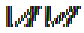
\includegraphics[width=\linewidth]{pics/truetype.png}
  \caption{stejné diagonály, TrueType render}
\end{figure}

\begin{figure}[H]
  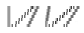
\includegraphics[width=\linewidth]{pics/truetype_bw.png}
  \caption{náhled intenzity svítivosti pixelů pří rendrování TrueType}
\end{figure}


\subsection{Kontura}
Střed písmen prochází hned o bod výš nad matematickým středem písmena, písmu tak spolu s netradičně seřezanými diagonály dodává dynamiku, která jde proti staticky řešeným písmům navrhovaným pro digitální zobrazování. Důležitým faktorem pro písmena v 1bitovém režimu je rovnoměrná distribuce pixelů, ideálně pod úhlem 45 stupňů a nebo pod jiným z bezpečných úhlů. Diagonály písmen se snaží držet úhel 45 stupňů horizontální-vertikální seřezávání diagonál usnadňuje práci s tímto úhlem a zároveň písmena nepřesahují svojí optickou šířku. Takto řešené konce diagonál dodávají písmu svou osobitost a jiný pohled na věc. Kontura nepotřebuje striktně držet mřížku ze které vychází. Potencionální digitální užití písma může být v případě mé práce primární ale určitě ne jediné, je důležité tedy myslet na to, aby písmo bylo kvalitní a originální v každé aplikaci. Písmo tedy musí splňovat i kvality které vyžadují tištěná média a digitální užití.
\subsection{Hinting}
Udržení rovnoměrné distribuce pixelů je velmi náročné při 1bitovém renderování, můžeme sami porovnat obr. 2 \& 3. Osa X disponuje v případě TrueTypu třikrát větším rozlišením, což nejsme schopni lehce na zařízeních pozorovat. Je důležité si vzpomenou, že pixel může být jakkoliv veliký a pozorován z jakékoliv vzdálenosti jak v kontextu tak bez kontextu. Subpixelu na monitoru počítače si nevšimneme, všimneme si ale subpixelu na velike LED instalaci, ke které můžeme přistoupit z jakékoliv vzdálenosti? Estetika písma vychází z části z nástrojů, kterým disponuje hintovací program VTT. Nastavit zde úhel nejde přímo, se vzdálenosti se ovšem dá pracovat několika způsoby. Známe-li vzdálenost dvou stran trojúhelníku, můžeme nastavit úhel diagonály pomocí nich. Tenhle způsob je limitován pouze dvěma věcmi. 1. je přehlednost pracovního souboru, pro každou vzdálenost si musíme do šuplíku vzdálenosti uložit jednu proměnou. Jestli je takových proměnných spoustu, je pravděpodobné, že nad proměnnými ztratíme přehled. 2. výška trojúhelníku je omezena ještě neznámou proměnnou - výškou dotažnic. Pro vertikální pohyb je tedy zapotřebí volný prostor pro natahování vertikální strany trojúhelníku. Jednoduše řečeno - výška diagonály natažené od účaří k výšce x je dána výškou x, nemůžeme jí tedy nastavit absolutní hodnotou.
\subsection{Prezentace a testování na displayích Nokia}
Nokia display 5110 je dostatečně otevřený na to abych se do něj dostal a zároveň je zástupcem jednobitových displejů na které se zaměřuji a proto to byla jasná volba pro prezentaci a testování mého písma Delta. Jako počítač pro vykreslování písmen používám Raspberry Pi Zero WH, na kterém běží program napsaný v Pythonu 3, který jako rasterizér používá knihovnu FreeType, výsledek je tedy totožný s tím jak by se písmo chovalo na zařízení které je postaveno na Linuxu. Testovat písmo právě na tomto rasterizéru je dobrou myslím dobrou volbou hlavně proto, že je velká možnost, že koncové užití písma bude právě na zařízení s tímto rasterizérem.
\subsection{Budoucnost mé bakalářské práce}
Projekt bych budu sdílet na Githubu a začnu postupně přidávat podporu dalších jazyků. Zkušenosti, které jsem nabral na latince bych rád aplikoval i do jiných písmových systémů, kde technologie nemusí být tak vyvinuta a potřeba dalšího současného písma s hintingem je potřeba.

\texcount 
\end{document}
